\section{Research Method}\label{sec:research_methods}

\subsection{GRATiS design}
The specific method used to achieve the design goal is to use GROOVE as a replacement of the STS in ATM. Figure~\ref{fig:tooling} shows this graphically. The \textbf{Test Manager} component communicates with an \textbf{STS Engine Interface}. This component obtains STS information from an \textbf{Exploration Strategy Interface} component, located at the GROOVE side. The \textbf{Rule Applier} component obtains the exploration strategy from the latter interface. The possible rule transitions are translated by the interfaces to possible switch relations for the Test Manager. The instantiated switch relation chosen is translated back to a rule transition by the interfaces. The exploration of the graph grammar is done \textit{on the fly}; rule transitions are explored only when chosen by the Test Manager. This is a setup for an on the fly model-based testing tool with on the fly model exploration. Note that this setup allows other tools to also communicate with these interfaces.

\begin{figure}[ht]
  \begin{center}
    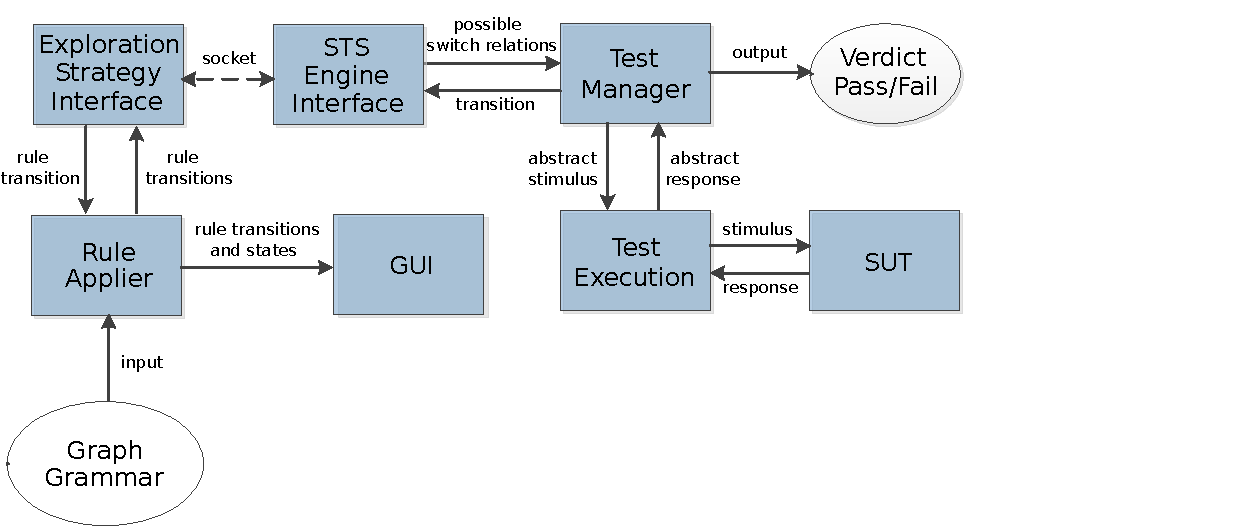
\includegraphics[width=\textwidth]{tooling.pdf}
  \end{center}
  \caption{The GRATiS design: replacing the STS with GROOVE}
  \label{fig:tooling}
\end{figure}

\subsubsection{Problems}\label{sec:problems}
The boardgame example revealed some problems, listed below, for the GRATiS design. These need to be tackled during the design phase of the project. 
\begin{itemize}
  \item Modelling data types such as integers and strings in GROOVE is problematic; the range of possible values has to be given explicitly. For example, it would be impossible to extend the die of the boardgame example such that it can throw any integer; each value of an integer would have to be defined separately.
  \item Coverage statistics cannot be calculated on GRATiS, if the model exploration is done on the fly. The number of states/locations and transitions/switch relations the model has when completely explored are not known, so a percentage cannot be derived.
\end{itemize}

\subsubsection{Initial design: GRATiS-Min}\label{sec:init_design}
Before the problems in~\ref{sec:problems} are tackled and the design of GRATiS implemented, an initial design that minimally achieves the design goal is implemented. This initial design, named GRATiS-Min performs the following steps:
\begin{enumerate}
  \item generate the GTS based on the graph grammar using GROOVE
  \item transform the GTS to an STS with the method described in section~\ref{sec:gts_sts_trafo}
  \item send the STS to ATM
  \item perform the automatic test generation on the STS
\end{enumerate}
This setup can be classified as on the model-based testing with \textit{offline} model exploration.

There are a number of advantages to GRATiS-Min:
\begin{enumerate}
  \item It allows automatic test generation on models which GROOVE is able to fully explore. This has been done on some interesting systems, as described in section~\ref{sec:descriptiongroove}.
  \item It is easy to implement. Only the transformation in section~\ref{sec:gts_sts_trafo} and a basic protocol for transmitting an STS need to be implemented.
  \item It can calculate coverage statistics, because the number of states and transitions are known. Note that the location and switch relation coverage is the same as graph state and rule transition coverage, as the transformation creates one location and one switch relation for each graph state and rule transition respectively. Therefore, we will call location and switch relation coverage statics not \textit{relevant} for suboptimal STSs.
  \item It already implements some features of GRATiS, such as the communication between GROOVE and ATM, which makes GRATiS easier to build.
\end{enumerate}
There are also some disadvantages:
\begin{enumerate}
  \item All states and transitions in the GTS need to be explored first. This is very costly in terms of time and memory.
  \item The test strategies of ATM do not work on the suboptimal STS. First of all, the strategy designed to obtain a high location/switch relation coverage will attempt to achieve a high graph state/rule transition coverage. The coverage on the reduced, optimal STS may therefore have been higher, as the strategy is satisfied by choosing switch relations it has already chosen with different data values (note that these are different switch relations in the suboptimal STS). Secondly, boundary-value analysis cannot be used, as each switch relation has one specific set of data values needed to enable the switch relation.
\end{enumerate}

\subsubsection{Solutions}
A tool with on-the-fly model exploration can not calculate coverage statistics, as clarified in section~\ref{sec:problems}. However, it does not suffer the disadvantages of GRATiS-Min, depending on whether graph states can be transformed to locations with location variables and the rule transitions to switch relations, such that the resulting STS is optimal. However, this transformation of a GTS to an optimal STS can also be applied to GRATiS-Min to solve the second disadvantage. This also makes location and switch relation coverage relevant. The first disadvantage can be solved by finding a transformation from a graph grammar to an STS, without constructing the GTS first. If such a transformation can be found, the resulting tool will be an on the fly model-based testing tool with offline model exploration and coverage statistics. If such a transformation cannot be found, this tool will be very costly in terms of time and memory. The alternative is an on the fly model-based testing tool with on the fly model exploration and no coverage statistics.

\subsection{GRATiS Validation}\label{sec:research_methods_validation}
There are two steps in the validation:
\begin{enumerate}
  \item The boardgame example is tested. A SUT is made for this game and ATM is used to test this game. Then, GRATiS is used to test the boardgame. The results should reveal no errors, fail verdicts or other differences in the output of both tools. An intentional error is then made in the SUT and the process is repeated. Still no errors or differences are expected, but both tools should find the error and give a fail verdict.
  \item Next, the assessment of the strengths and weaknesses of GRATiS is done by applying both tools to several case studies and comparing the results. The case studies are set out first and then the criteria for the comparison are given.
\end{enumerate}

\subsubsection{Case studies}
Three case studies are planned. They are all real-life systems Axini has worked on:
\begin{itemize}
  \item a self-scan register
  \item a navigation system
  \item a health-care system
\end{itemize}  

The self-scan register is a machine that automates the purchase of products at a supermarket. A customer can put his products on a conveyer belt and the system automatically calculates the price of the products. Then the customer pays and gets a receipt. The navigation system is a GPS device with a route planner. It allows a user to enter a destination and the system plans the correct route accordingly from the location of the user. The health-care system is a medical device.

A GTS and an STS will be created for each system. GRATiS and ATM are used for the automatic test generation on these models respectively. Both the model and the test process will then be compared as part of the validation. The next two sections give the criteria for this comparison.

\subsubsection{Objective criteria}
As mentioned in section~\ref{sec:questions}, the criteria for the comparison of ATM and GRATiS are split in two parts. The objective criteria that can be compared are:
\begin{enumerate}
  \item The verdicts: same test cases should give same verdicts. When a verdict is different for the same test case in GRATiS and ATM, this might indicate an error.
  \item The number of bugs found: one tool could generate smarter test-cases and find more bugs.
  \item The coverage: generating smarter test-cases can also lead to a higher coverage.
  \item The test cases generated per second: benchmarks will be done on how fast the tools generate test-cases.
  \item The size of the statespace: benchmarks will be done on how much space the tools use.
\end{enumerate}

\subsubsection{Subjective criteria}
Subjective criteria, such as the maintainability and extendibility of a model, are related to the usability of GTSs versus alternative formalisms, such as STSs. Evaluaiting such criteria requires an extensive experiment with a statistical significant set of human actors. It is out of the scope of this project to perform such an experiment in order to compare two modelling formalisms. In section~\ref{sec:introduction} a motivation is given for the use of GTSs in model-based testing. The qualities of GTSs described there cover the usability of the GTSs.
